\subsection{Erstellung des Raspberry PI \textit{Images}}
Technikerinnen und Techniker müssen die Schritte zum Aufsetzen eines Raspberry PIs (siehe Kapitel \ref{raspi_setup}) bei einer Neuinstallation nicht durchführen, da ihnen ein vorgefertigtes \gls{image} verabreicht wird. Dieses muss lediglich auf die SD-Karte des Raspberry PIs kopiert und nicht weiter konfiguriert werden. Die Erstellung dieses \gls{image}\textit{s} wird folgend erläutert.

Das \gls{image} wird über einen Computer mit Linux erstellt, daher kommt eine \ac{vm} zum Einsatz, um einfach eine Linux Distribution auf einem Windows Computer laufen zu lassen. Dabei können unterschiedliche Linux Distributionen verwendet werden, wobei mindestens 4 Gigabyte Arbeitsspeicher, 2 Prozessorkerne und 80 Gigabyte Festplattenspeicher empfohlen werden. 

\paragraph{\textit{Image} klonen}
Das \gls{image} wird erstellt, indem ein Speicherabbild einer SD-Karte mit funktionierendem Betriebssystem und \gls{gls_python} Programm gemacht wird. Dieser Prozess findet hauptsächlich in der Kommandozeile statt, daher muss das Linux-Terminal geöffnet werden, um die folgenden Befehle auszuführen:
\begin{enumerate}
    %\item Zur Vorbereitung wird GParted mit \mintinline{console}{sudo apt-get install gparted} installiert. 

    \item Um die SD-Karte zu klonen, muss zuerst ihr Pfad mithilfe des Befehls \mintinline{console}{sudo fdisk -l} ermittelt werden. Dabei ist in Abb. \ref{fig:sudo_fdisk} zu sehen, dass der Pfad in diesem Beispiel \enquote{dev/sdb} ist.
    \begin{figure}[H]
        \centering
        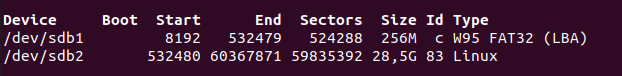
\includegraphics[width=0.75\linewidth]{sudo_fdisk}
        \caption{Ergebnis des \mintinline{console}{sudo fdisk -l} Befehls im Linux Terminal}
        \label{fig:sudo_fdisk}
    \end{figure}
    
    \item Im nächsten Schritt kann die SD-Karte geklont werden. Dazu wird der Befehl \mintinline{console}{dd} verwendet, wobei bei \mintinline{console}{if=} das input file \bzw der Pfad der SD-Karte angegeben wird und bei \mintinline{console}{of=} das output file \bzw der Pfad der \gls{image} (\enquote{.img}) Datei angegeben wird:
    \begin{minted}{console}
sudo dd if=/dev/sdb of=/home/ubuntu/Desktop/clone.img
    \end{minted}

    \item Da die aus dem vorgehenden Befehl generierte \gls{image} Datei mehr als 30 Gigabyte groß ist, kann das \enquote{PyShrink} Skript verwendet werden, um das große  \gls{image} auf etwa 5 bis 6 Gigabyte zu verkleinern. \enquote{PyShrink} wird mit den folgenden Befehlen über die Kommandozeile installiert:
    \begin{minted}[breaklines=true, breakanywhere=true]{console}
wget https://raw.githubusercontent.com/Drewsif/PiShrink/master/pishrink.sh
chmod +x pishrink.sh
sudo mv pishrink.sh /usr/local/bin
    \end{minted}

    Nach der Installation, kann das \gls{image} mithilfe des nachfolgenden Befehls verkleinert werden. Hier wird ebenfalls zuerst der Pfad der Eingabedatei und dann der Pfad der Ausgabedatei angegeben:
    \begin{minted}[breaklines=true, breakanywhere=true]{console}
sudo pishrink.sh /home/ubuntu/Desktop/clone.img /home/ubuntu/Desktop/shrunken-image.img
    \end{minted}

    \item Das verkleinerte Image kann nun auf eine neue SD-Karte geflasht werden. Dafür kann ein beliebiger Imager, wie \zB \enquote{balenaEtcher} \enquote{Win32DiskImager} oder \enquote{RaspberryPi-Imager}, genutzt werden.
\end{enumerate}



